\documentclass[8pt,a4paper,compress]{beamer}

\usepackage{/home/siyer/lib/slides}

\title{Shortest Paths}
\date{}
\begin{document}
\begin{frame}
\vfill
\titlepage
\end{frame}

\begin{frame}
\frametitle{Outline}
\tableofcontents
\end{frame}

\section{Shortest Paths}
\begin{frame}[fragile]
\pause

A shortest path from vertex $s$ to vertex $t$ in an edge-weighted digraph is a directed path from $s$ to $t$ with the property that no other such path has a lower weight

\pause
\bigskip

An edge-weighted graph and a shortest path
\begin{minipage}{150pt}
\begin{lstlisting}[language={}]
$ more tinyEWD.txt 
8
15
4 5 0.35
5 4 0.35
4 7 0.37
5 7 0.28
7 5 0.28
5 1 0.32
0 4 0.38
0 2 0.26
7 3 0.39
1 3 0.29
2 7 0.34
6 2 0.40
3 6 0.52
6 0 0.58
6 4 0.93
\end{lstlisting}
\end{minipage}%
\begin{minipage}{150pt}
\begin{center}
\visible<3->{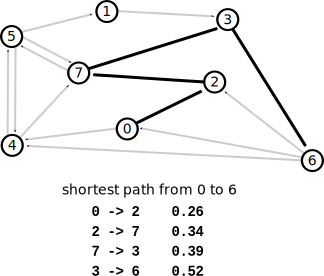
\includegraphics[scale=0.45]{{./figures/sp1}.pdf}}
\end{center}
\end{minipage}
\end{frame}

\begin{frame}[fragile]
\pause

Variants: single source, single sink, source-sink, all pairs

\pause
\bigskip

Typical shortest-paths applications
\begin{center}
\begin{tabular}{ccc}
application & vertex & edge \\ \hline
map & intersection & road \\
network & router & connection \\
schedule & job & precedence constraint \\
arbitrage & currency & exchange rate
\end{tabular}
\end{center}
\end{frame}

\section{Edge-Weighted Digraph API}
\begin{frame}[fragile]
\pause

Weighted directed edge data type (API)
\begin{center}
\begin{tabular}{cc}
method & description \\ \hline
\lstinline$DirectedEdge(int v, int w, double weight)$ & create a directed weighted edge $v$-$w$ \\
\lstinline$int from()$ & vertex this edge points from \\
\lstinline$int to()$ & vertex this edge points to \\
\lstinline$double weight()$ & weight of this edge
\end{tabular}  
\end{center}

\pause
\bigskip

Weighted directed edge data type (implementation)
\begin{lstlisting}[language=Java]
package edu.princeton.cs.algs4;

public class DirectedEdge { 
    private final int v;
    private final int w;
    private final double weight;
    
    public DirectedEdge(int v, int w, double weight) {
        if (v < 0 || w < 0) { throw new IndexOutOfBoundsException(); }
        if (Double.isNaN(weight)) { throw new IllegalArgumentException(); }
        this.v = v;
        this.w = w;
        this.weight = weight;
    }

    public int from() { return v; }

    public int to() { return w; }

    public double weight() { return weight; }
}
\end{lstlisting}
\end{frame}

\begin{frame}[fragile]
\pause

Edge-weighted digraph (API)
\begin{center}
\begin{tabular}{cc}
method & description \\ \hline
\lstinline$EdgeWeightedDigraph(int V)$ & edge-weighted digraph with $V$ vertices \\
\lstinline$EdgeWeightedDigraph(In in)$ & edge-weighted digraph from input stream \\
\lstinline$void addEdge(DirectedEdge e)$ & add weighted directed edge $e$ \\
\lstinline$Iterable<DirectedEdge> adj(int v)$ & edges pointing from $v$ \\
\lstinline$int V()$ & number of vertices \\
\lstinline$int E()$ & number of edges \\
\end{tabular}  
\end{center}
\end{frame}

\begin{frame}[fragile]
\pause

Edge-weighted digraph (implementation)
\begin{lstlisting}[language=Java]
package edu.cs.princeton.algs4;

public class EdgeWeightedDigraph {
    private final int V;
    private int E;
    private LinkedBag<DirectedEdge>[] adj;
    
    public EdgeWeightedDigraph(int V) {
        if (V < 0) { throw new IllegalArgumentException(); }
        this.V = V;
        this.E = 0;
        adj = (LinkedBag<DirectedEdge>[]) new LinkedBag[V];
        for (int v = 0; v < V; v++) {
            adj[v] = new LinkedBag<DirectedEdge>();
        }
    }

    public EdgeWeightedDigraph(In in) {
        this(in.readInt());
        int E = in.readInt();
        if (E < 0) { throw new IllegalArgumentException(); }
        for (int i = 0; i < E; i++) {
            int v = in.readInt();
            int w = in.readInt();
            double weight = in.readDouble();
            addEdge(new DirectedEdge(v, w, weight));
        }
    }
    
    public int V() { return V; }

    public int E() { return E; }
\end{lstlisting}
\end{frame}

\begin{frame}[fragile]
\pause

\begin{lstlisting}[language=Java]
    public void addEdge(DirectedEdge e) {
        int v = e.from();
        int w = e.to();
        validateVertex(v);
        validateVertex(w);
        adj[v].add(e);
        E++;
    }

    public Iterable<DirectedEdge> adj(int v) {
        validateVertex(v);
        return adj[v];
    }

    public Iterable<DirectedEdge> edges() {
        LinkedBag<DirectedEdge> list = new LinkedBag<DirectedEdge>();
        for (int v = 0; v < V; v++) {
            for (DirectedEdge e : adj(v)) {
                list.add(e);
            }
        }
        return list;
    } 
}
\end{lstlisting}
\end{frame}

\section{Shortest Path API}
\begin{frame}[fragile]
\pause

Single-source shortest paths API
\begin{center}
\begin{tabular}{cc}
method & description \\ \hline
\lstinline$SP(EdgeWeightedDigraph G, int s)$ & constructor \\
\lstinline$double distTo(int v)$ & distance from $s$ to $v$, $\infty$ if no path \\
\lstinline$boolean hasPathTo(int v)$ & path from $s$ to $v$? \\
\lstinline$Iterable<DirectedEdge> pathTo(int v)$ & path from $s$ to $v$, \lstinline$null$ if none
\end{tabular}  
\end{center}

\pause

SP test client
\begin{lstlisting}[language=Java]
package edu.princeton.cs.algs4;

public class DijkstraSP {
    public static void main(String[] args) {
       In in = new In(args[0]);
        EdgeWeightedDigraph G = new EdgeWeightedDigraph(in);
        int s = Integer.parseInt(args[1]);
        DijkstraSP sp = new DijkstraSP(G, s);
        for (int t = 0; t < G.V(); t++) {
            if (sp.hasPathTo(t)) {
                StdOut.printf("%d to %d (%.2f)  ", s, t, sp.distTo(t));
                if (sp.hasPathTo(t)) {
                    for (DirectedEdge e : sp.pathTo(t)) {
                        StdOut.print(e + "   ");
                    }
                }
                StdOut.println();
            }
            else { StdOut.printf("%d to %d         no path\n", s, t); }
        }
    }
}
\end{lstlisting}
\end{frame}

\begin{frame}[fragile]
\pause

\begin{lstlisting}[language={}]
$ java edu.princeton.cs.algs4.DijkstraSP tinyEWD.txt 0
0 to 0 (0.00):
0 to 1 (1.05): 0->4 0.38 4->5 0.35 5->1 0.32
0 to 2 (0.26): 0->2 0.26
0 to 3 (0.99): 0->2 0.26 2->7 0.34 7->3 0.39
0 to 4 (0.38): 0->4 0.38
0 to 5 (0.73): 0->4 0.38 4->5 0.35
0 to 6 (1.51): 0->2 0.26 2->7 0.34 7->3 0.39 3->6 0.52
0 to 7 (0.60): 0->2 0.26 2->7 0.34
\end{lstlisting}
\end{frame}

\begin{frame}[fragile]
\pause

A shortest-paths tree solution (SPT) always exists

\pause
\bigskip

Data structures: can represent the SPT with two vertex-indexed arrays
\begin{itemize}
\item \lstinline{distTo[v]} is length of shortest path from $s$ to $v$

\item \lstinline{edgeTo[v]} is last edge on shortest path from $s$ to $v$
\end{itemize}

\begin{center}
\visible<3->{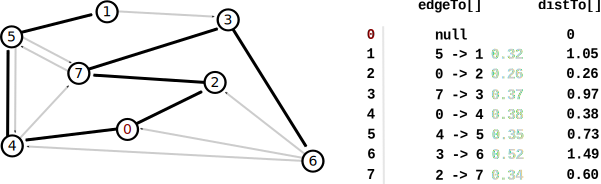
\includegraphics[scale=0.45]{./figures/sp2.pdf}}
\end{center}

\pause
\bigskip

Edge relaxation: relax edge $e = v\to w$
\begin{itemize}
\item \lstinline{distTo[v]} is length of shortest known path from $s$ to $v$

\item \lstinline{distTo[w]} is length of shortest known path from $s$ to $w$

\item \lstinline{edgeTo[w]} is last edge on shortest known path from $s$ to $w$

\item if $e = v\to w$ gives shorter path to $w$ through $v$, update both \lstinline{distTo[w]} and \lstinline{edgeTo[w]}
\end{itemize}
\end{frame}

\begin{frame}[fragile]
\pause

Edge relaxation (implementation)
\begin{lstlisting}[language=Java]
private void relax(DirectedEdge e) {
    int v = e.from(), w = e.to();
    if (distTo[w] > distTo[v] + e.weight()) {
        distTo[w] = distTo[v] + e.weight();
        edgeTo[w] = e;
    }
}
\end{lstlisting}

\pause
\bigskip

Edge relaxation (two cases)
\begin{center}
\visible<3->{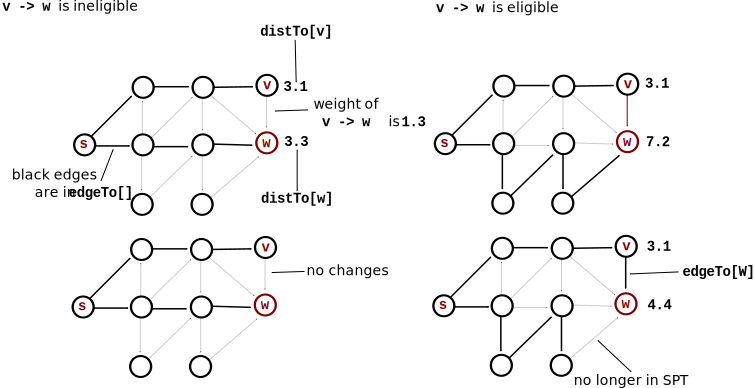
\includegraphics[scale=0.45]{./figures/sp3.pdf}}
\end{center}
\end{frame}

\section{Dijkstra's Algorithm}
\begin{frame}[fragile]
\pause

Dijkstra's algorithm computes a SPT in any edge-weighted
digraph with nonnegative weights, as follows

\begin{itemize}
\item Considers vertices in increasing order of distance from $s$ (non-tree vertex with the lowest \lstinline{distTo[]} value)
\item Adds vertex to tree and relaxes all edges pointing from that vertex
\end{itemize}

\pause
\bigskip

Implementation
\begin{lstlisting}[language=Java]
package edu.princeton.cs.algs4;

public class DijkstraSP {
    private double[] distTo; 
    private DirectedEdge[] edgeTo; 
    private IndexMinPQ<Double> pq; 
    
    public DijkstraSP(EdgeWeightedDigraph G, int s) {
        for (DirectedEdge e : G.edges()) {
            if (e.weight() < 0) { throw new IllegalArgumentException(); }
        }
        distTo = new double[G.V()];
        edgeTo = new DirectedEdge[G.V()];
        for (int v = 0; v < G.V(); v++) { 
            distTo[v] = Double.POSITIVE_INFINITY; 
        }
        distTo[s] = 0.0;
        pq = new IndexMinPQ<Double>(G.V());
        pq.insert(s, distTo[s]);
        while (!pq.isEmpty()) {
            int v = pq.delMin();
            for (DirectedEdge e : G.adj(v)) { relax(e); }
        }
    }    
\end{lstlisting}
\end{frame}

\begin{frame}[fragile]
\pause

\begin{lstlisting}[language=Java]
    public double distTo(int v) { 
        return distTo[v]; 
    }

    public boolean hasPathTo(int v) { 
        return distTo[v] < Double.POSITIVE_INFINITY; 
    }
    
    public Iterable<DirectedEdge> pathTo(int v) {
        if (!hasPathTo(v)) { return null; }
        LinkedStack<DirectedEdge> path = 
            new LinkedStack<DirectedEdge>();
        for (DirectedEdge e = edgeTo[v]; e != null; 
            e = edgeTo[e.from()]) {
            path.push(e);
        }
        return path;
    }
}
\end{lstlisting}

\pause
\bigskip

Dijkstra's algorithm using a binary heap based priority queue computes a SPT in an edge-weighted digraph in time proportional to $E\log V$ in the worst case
\end{frame}

\begin{frame}[fragile]
\pause

Trace
\begin{center}
\visible<2->{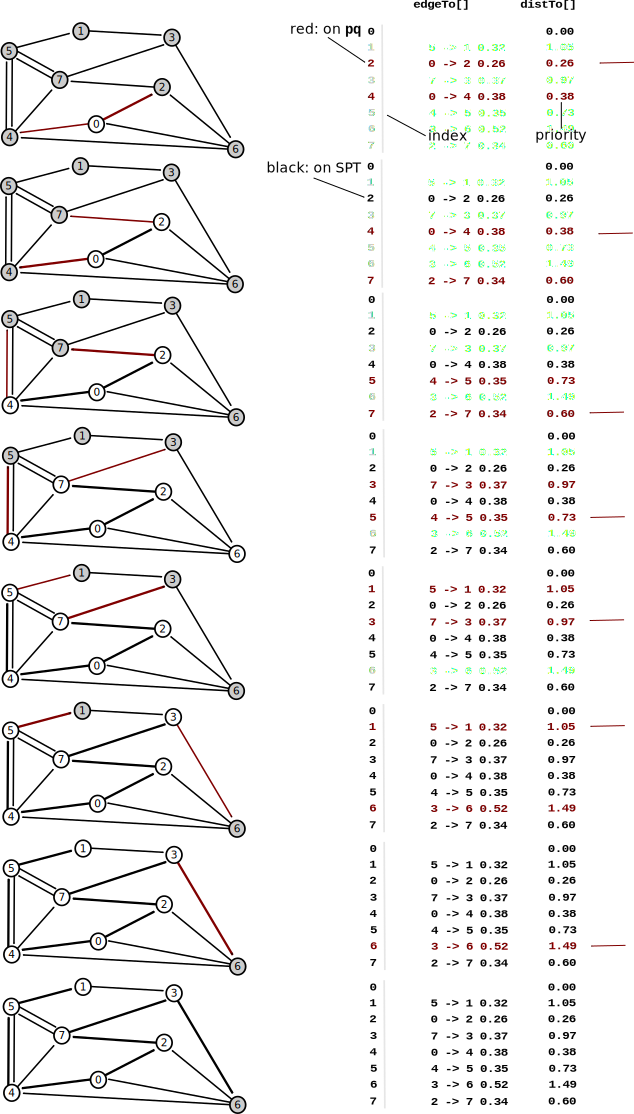
\includegraphics[scale=0.27]{./figures/sp4.pdf}}
\end{center}
\end{frame}

\section{Edge-Weighted DAGs}
\begin{frame}[fragile]
\pause

It is easier to find shortest paths in an edge-weighted DAG than in a general digraph
\begin{itemize}
\item Consider vertices in topological order

\item Relax all edges pointing from that vertex
\end{itemize}

\pause
\bigskip

Topological sort algorithm computes SPT in any edge-weighted DAG in time proportional to $E + V$

\pause
\bigskip

Implementation
\begin{lstlisting}[language=Java]
package edu.princeton.cs.algs4;

public class AcyclicSP {
    private double[] distTo; 
    private DirectedEdge[] edgeTo; 
    
    public AcyclicSP(EdgeWeightedDigraph G, int s) {
        distTo = new double[G.V()];
        edgeTo = new DirectedEdge[G.V()];
        for (int v = 0; v < G.V(); v++) {
            distTo[v] = Double.POSITIVE_INFINITY;
        }
        distTo[s] = 0.0;
        Topological topological = new Topological(G);
        if (!topological.hasOrder()) { 
            throw new IllegalArgumentException(); 
        }
        for (int v : topological.order()) {
            for (DirectedEdge e : G.adj(v)) { relax(e); }
        }
\end{lstlisting}
\end{frame}

\begin{frame}[fragile]
\pause

\begin{lstlisting}[language=Java]
    public double distTo(int v) { 
        return distTo[v]; 
    }

    public boolean hasPathTo(int v) { 
        return distTo[v] < Double.POSITIVE_INFINITY; 
    }
    
    public Iterable<DirectedEdge> pathTo(int v) {
        if (!hasPathTo(v)) { return null; }
        LinkedStack<DirectedEdge> path = 
            new LinkedStack<DirectedEdge>();
        for (DirectedEdge e = edgeTo[v]; e != null; 
            e = edgeTo[e.from()]) {
            path.push(e);
        }
        return path;
    }
}
\end{lstlisting}
\end{frame}

\begin{frame}[fragile]
\pause

Trace
\begin{center}
\visible<2->{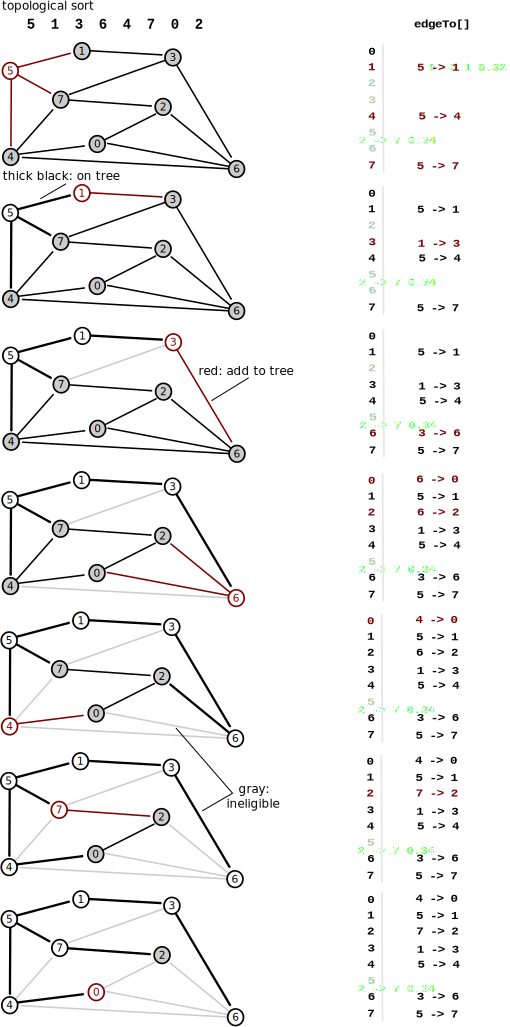
\includegraphics[scale=0.28]{./figures/sp5.pdf}}
\end{center}
\end{frame}

\section{Summary}
\begin{frame}[fragile]
\pause

Nonnegative weights
\begin{itemize}
\item Arise in many applications
\item Dijkstra's algorithm is nearly linear-time
\end{itemize}

\pause
\bigskip

Acyclic edge-weighted digraphs
\begin{itemize}
\item Arise in some applications
\item Topological sort algorithm is linear time
\item Edge weights can be negative
\end{itemize}

\pause
\bigskip

Negative weights and negative cycles
\begin{itemize}
\item Arise in some applications
\item If no negative cycles, can find shortest paths using Bellman-Ford algorithm
\item If negative cycles, can find one using Bellman-Ford algorithm
\end{itemize}

\pause
\bigskip

Shortest-paths is a broadly useful problem-solving model
\end{frame}
\end{document}
